\section{Introduction} Predicting nucleic acid binding sites on protein structures is an important computational task.  There are many existing methods which attempt to solve this problem either on the sequence level or on 3D structure level based on either sequence features or structural features of proteins \citep{deng2018pdrlgb, wang2010bindn+, wang2006bindn, li2013predna}.
We represent protein surfaces as 3D triangulated meshes with 
vertices and edges having features representing different geometrical and physicochemical aspects of the protein structure. Now, we can learn a model which classifies each vertex of such a mesh to either binding-site or
non-binding sites. With recent advances in 3D deep learning, Graph Convolutional
Networks(GCNs) have come out as a useful approach for learning higher level features over
3D mesh objects. We developed a GCN based deep learning model for the binding site classification
task: PNAbind. \hyperref[fig:crf_concept]{Fig. 1.1A} shows a schematic diagram of
the task PNAbind achieves.

Standard neural network approach is to predict each binding-site label independently
through it's output layer. However, classification tasks often come with additional non-trivialities which
are not addressable with independence assumption.  For example, image segmentation task involves
classifying every pixel of an image (which can be thought of as a grid of pixels) to some class.
However, independence assumption often gives poor/scattered results. In that case, some form of
conditional label (re)assignment is necessary for each pixel considering its neighbouring pixels. The
most common way to achieve the same in the field of computer vision is via optimizing a conditional
random  field (CRF) model over a set of initially  learned labels. For example,
\hyperref[fig:crf_concept]{Fig. 1.1B} adapted
from \citet{krahenbuhl2012efficient}  shows how an implementation based on CRF can improve image
segmentation results. In our case, we also expect certain properties from a predicted binding site
region on a protein surface. A binding site region on a protein surface is a combination
of multiple mesh vertices predicted as binding sites. We generally expect such a region to be
"smooth" i.e. not randomly have misclassified points scattered around. This idea is visually illustrated in
\hyperref[fig:crf_concept]{Fig. 1.1C}. So, we need to do some kind
of conditional (re)assignment of class labels generated by PNAbind.

In addition to Computer vision, CRF models are also heavily used in Natural Language processing (NLP)
\citep{roark2004discriminative,mccallum2003early,liu2017identification}. However, both in Computer vision and NLP, the underlying graph structure, over which the CRF is defined, is very sparse and simple e.g. linear chain or tree for NLP and 2D grid for computer vision. Which makes it easy to
find some form of optimization scheme on the discrete domain of labels. However, this is not the
case for a general underlying graph, where the combinatoriality of the possible label assignments
for all vertices is huge and in the discrete domain of labels there is no gradient information for
efficient optimization.

\citet{krahenbuhl2012efficient} proposes an efficient inference algorithm for fully connected CRFs
based on mean field Variational Inference and high dimensional filtering using permutohedral lattice
approximation. However, the high dimensional filtering step is not compatible with
SIMD\citep{nickolls2008scalable} paradigm of GPU computation. \citep{teichmann2018convolutional}
making it impossible to use on large datasets and non-trivial graphs.
\citet{teichmann2018convolutional} improves upon this by implementing Convolutional CRFs which is
another kind of approximation to full CRF inference which is efficient and compatible with GPUs.
However, their method is only applicable for 2D grid i.e. image data.  However, none of these methods
are applicable to our case directly. One of the more interesting advances of applying a CRF layer on
mesh objects comes from \citet{kalogerakis2010learning} using alpha-expansion graph-cuts method proposed by
\citet{boykov2001fast}. However, being pre-CNN revolution work, this method is not suitable for deep
learning and is not readily integrable to our PNAbind model. 
\par
Overall, it turns out, optimizing a CRF model over the predicted labels of PNAbind on the discrete domain to reassign them is not computationally expensive. However, instead of trying to smooth the predicted labels, we can directly try to make these predicted labels itself smoother. This means we need to have an operation before the final fully connected layer of PNAbind which smooths the information over different vertices taking into account their neighbours information along with their own. The good thing about this idea is that the optimization domain is not discrete anymore.

Such an operation is based on a continuous variant of a CRF or CCRF. \citet{ristovski2013continuous}
shows how to calculate the updates for such a model using mean field variational inference, although
not in a neural network context. \citet{gao2019conditional} introduces this approach for graph convolution based networks, however, the network layer update equation presented in their work results in simply an Identity transformation. We calculated the correct
form of the network layer which we can be used as the second last layer of PNAbind.

In next sections, we shall formally describe a metric denoting ``smoothness" of binding site prediction over protein meshes, the CCRF model and the CCRF layer's architecture, followed by results showing how it has significantly improved PNAbind for the binding site classification task.
\begin{center} 
 \begin{figure}[!htp]
                \makebox[\textwidth]{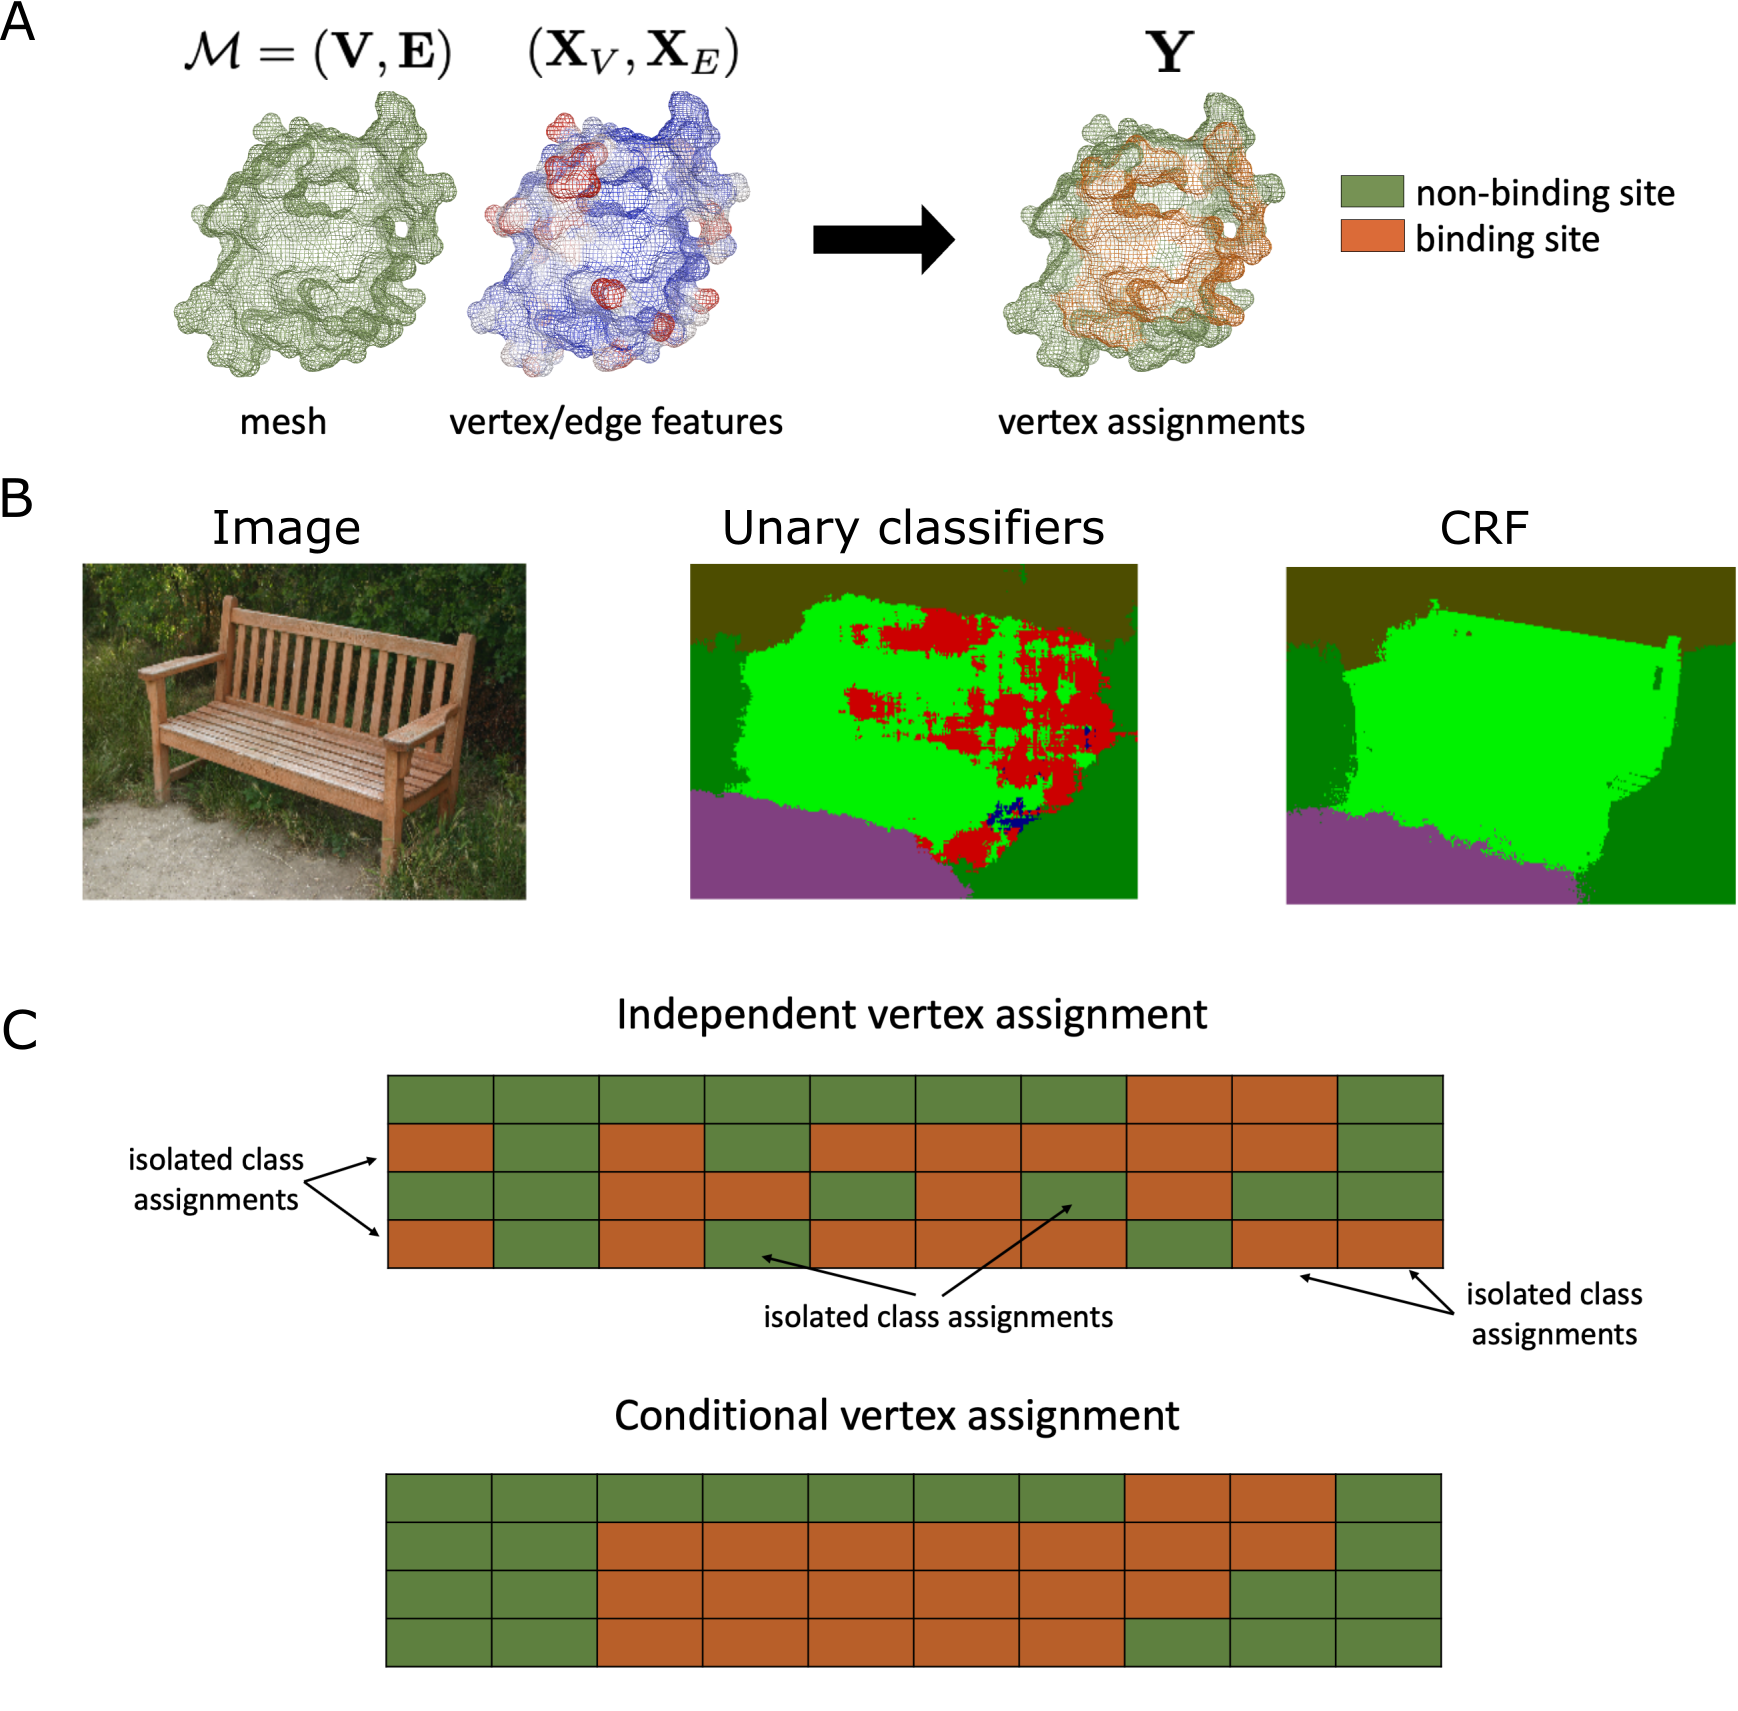
\includegraphics[width=0.8\paperwidth]{crffigs/crf_concept.png}}
 % archetecture.png: 1149x508 px, 72dpi, 40.53x17.92 cm, bb=0 0 1149 508
        \caption[PNAbind schematic, example and conceptual explanation of CRF application scenario]{\textbf{PNAbind schematic, example and conceptual explanation of CRF application scenario}
        ({\bf A}) Schematic diagram showing how PNAbind predicts binding sites over a protein surface represented as a mesh. ({\bf B}) \citet{krahenbuhl2012efficient} shows how applying a fully connected CRF model results in better image segmentation results compared to 
        just unary classification. ({\bf C}) (above) An example independent class assignment in a 2-D grid of cells which is irregular, (below) A smoother classification, which we would 
        expect to get as result of a conditional assignment process.}
        \label{fig:crf_concept} \end{figure} \end{center}
